\section{Kontrolfunktioner}
\underline{\textbf{Controller klassen}}
\newline
Der blev valgt at samle programmets vigtigste funktioner i klassen \texttt{Controller}. Dette blev gjort for at user interface kun skulle i kontakt med én klasse, og fordi det ville blive nemmere i en senere iteration at implementere et Grafisk User Interface (GUI).
\newline
En af \texttt{Controller} klassens metoder er \texttt{sendBesked(besked, uName)}. Samarbejdsdiagrammet for \texttt{sendBesked()} er vist i figur \ref{fig:sendb}.
\begin{figure}[ht]
	\centering
	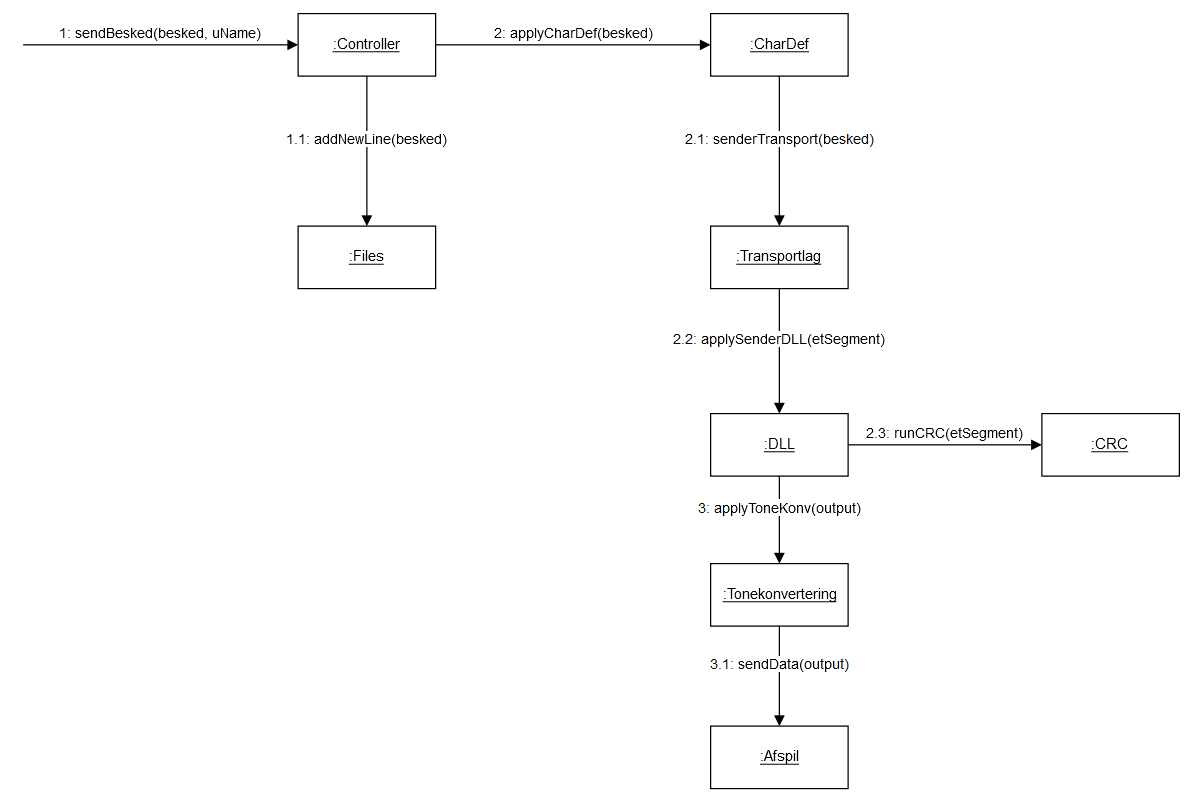
\includegraphics[width=15cm,height=25cm,keepaspectratio]{pictures/SDsend.png}
	\caption{\texttt{sendBesked()}}
	\label{fig:sendb}
\end{figure}
\hfill \break
Denne metode tager beskeden der skal sendes, samt navnet på den der har sendt den og samler det i en besked. Denne besked bliver sendt videre til \texttt{Chardefinition} klassen, som laver teksten om til en binær streng. Den bliver efterfølgende sendt til transportlaget, der kan dele beskeden op i mindre segmenter og sørge for at sendingerne foregår som de skal. Pakkerne vil kommere videre til Data Link Laget, hvor der vil blive tilføjet CRC og stuffing til bitstrengen. I \texttt{Tonekonvertering} bliver den binære streng omdannet til tal mellem 0 og 15, som er det antal toner der er til rådighed ved DTMF. Til sidst bliver tonerne afspillet med klassen \texttt{Afspil}. Når en besked er sendt, bliver den gemt i en fil med klassen \texttt{Files}.
\newline
Klassen har desuden en metode, der hedder \texttt{modtagBesked(uName)}. Samarbejdsdiagrammet for \texttt{modtagBesked()} er vist i figur \ref{fig:modtagb}.
\begin{figure}[ht]
	\centering
	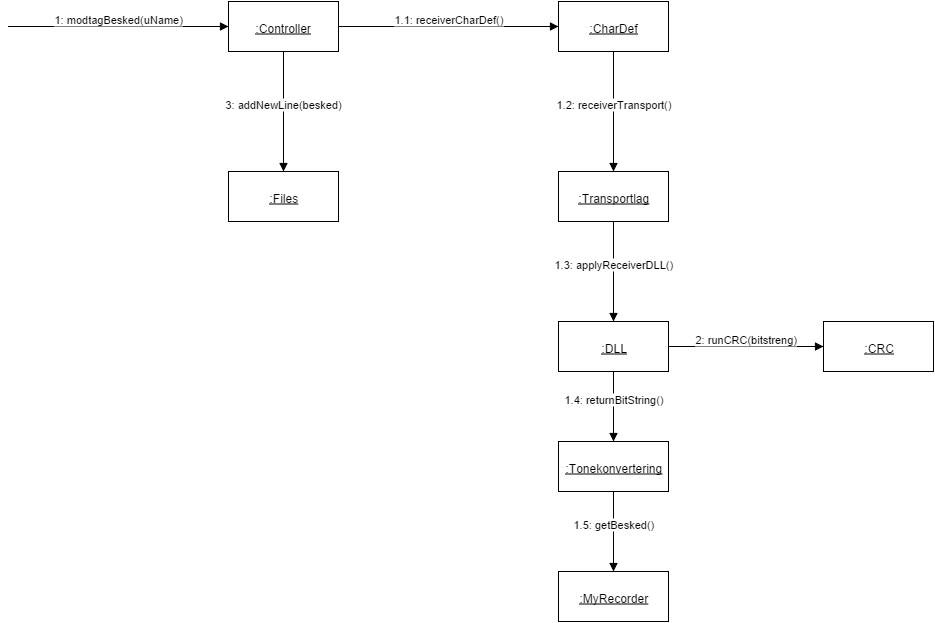
\includegraphics[width=15cm,height=25cm,keepaspectratio]{pictures/SDmodtagBesked.png}
	\caption{\texttt{modtagBesked()}}
	\label{fig:modtagb}
\end{figure}
\hfill \break
Denne går igennem de samme klasser som \texttt{sendBesked}, dog i stedet for at sende en besked afsted, sendes der en request om at modtage en besked. I klassen \texttt{MyRecorder} modtages beskeden, som returneres som toner af tal mellem 0 og 15 til \texttt{Tonekonvertering}'en, der omdanner tonerne til en bitstreng, som returneres til Data link laget. Ved \texttt{DLL} tjekkes for CRC og stuffing fjernes inden det returneres til transportlaget, hvor beskeden sættes sammen igen, hvis beskeden var delt op i segmenter. Den kommer retur til \texttt{CharDef} og bliver lavet fra binær streng til karakterer, som derefter returneres til \texttt{Controller}, der viser beskeden på skærmen og samtidig bruger \texttt{Files} til at gemme beskeden i en historik. Til dette bruges \texttt{uName} i metoden for at gemme i den rigtige historik.
\newline
\texttt{testLogin(uName, pWord)} er metoden der kan teste om et brugernavn og password er korrekt. Dette gør den ved at bruge \texttt{Login} klassen.
\newline
\texttt{createUser(uName, pWord)} bruger igen \texttt{Login} klassen, denne gang til at oprette en bruger. Samarbejddiagrammet er vist i figur \ref{fig:createu}.
\begin{figure}[ht]
	\centering
	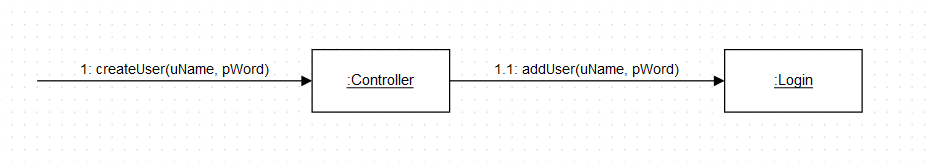
\includegraphics[width=15cm,height=25cm,keepaspectratio]{pictures/SDcreateUser.png}
	\caption{\texttt{createUser()}}
	\label{fig:createu}
\end{figure}
\hfill \break

Der er også metoder der kan vise historikken. De bruger alle \texttt{Files} klassen og kan enten vise hele historikken, sidste besked eller en der kan definere hvor mange linjer der skal hentes og vises.
